\section{Approach and Uniqueness\label{sec:approach}}
\begin{figure}
    \begin{center}
        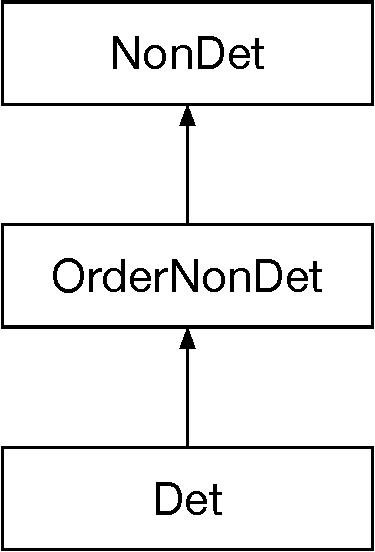
\includegraphics[scale=0.37]{detHierarchy}
    \end{center}
    \caption{Determinism type qualifier hierarchy}
    \label{fig:determinism-hierarchy}
\end{figure}

The core of the determinism type system is the following type qualifiers:
\begin{itemize}
    \item \<NonDet> indicates
    that the expression might have different values in two different executions.
    \item \<OrderNonDet> indicates that the expression is a collection or
    a map that contains the same elements in every execution, but possibly
    in a different order.
    \item \<Det> indicates that the expression evaluates to equal values in
    all executions; for a collection, iteration
    also yields the values in the same order.
\end{itemize}
\Cref{fig:determinism-hierarchy} shows the subtyping
relationship among the qualifiers.

Programmers can write these type qualifiers to specify their program's behavior.
\<OrderNonDet> may only be written on collections and maps.
A map is a dictionary or an associative array, such as a hash table.
\OurTypeSystem largely treats a map as a collection of key--value pairs.
Both collections and maps may be \<Det>, \<OrderNonDet>, or \<NonDet>.
The basetypes of their elements can be specified independently of the collection basetypes.
However, an element type qualifier must be a subtype of the collection type qualifier.

\subsubsection{Behavior of order-nondeterministic collections}\label{sec:ond-behavior}
A collection of type \<OrderNonDet> has special properties, including the following.

\begin{enumerate}
    \item
    The individual elements retrieved from it have type \<NonDet>.  This
    affects access, iteration, searching, etc.
    \item
    Size-related operations return a deterministic result.  This also affects
    queries of whether an iterator has more elements.
    \item
    If the collection is sorted, or its elements are placed in a collection
    that does sorting, the result is deterministic.
\end{enumerate}
